\chapter{Web Server - Workload Characterization}
\begin{figure}[H]
	\centering
	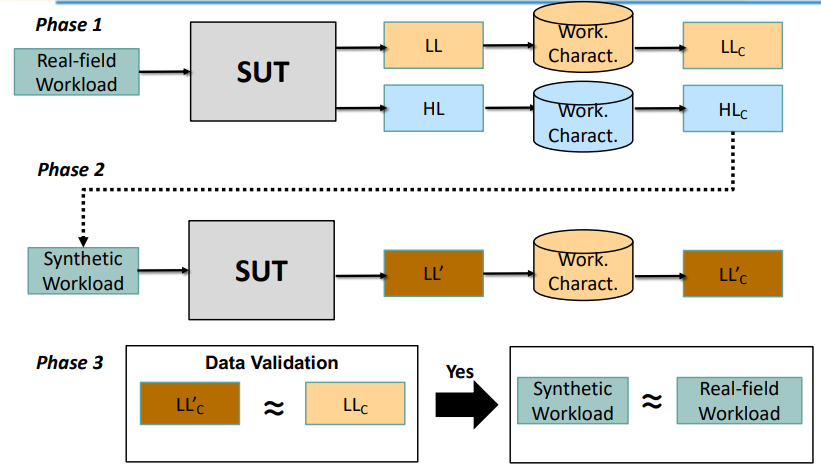
\includegraphics[width=0.5\textwidth]{img/hw3/Overview.png}
	\caption{\textit{Overview WL Characterization}}
\end{figure}
\section{Real-field Workload}
Generazione workload reale random
\\
Collezionamento parametri alto e basso livello
\\
Caratterizzazione parametri alto livello e generazione workload sintentico
\\
DA QUA INIZIO IO
\\
Caratterizzazione parametri basso livello wl reale
\section{Synthetic Workload}
Collezionamento parametri basso livello wl sintetico
\\
Caratterizzazione parametri basso livello wl sintetico
\\
Random Selection su entrambi per identificare l'elemento rappresentativo di ogni cluster
\section{Data Validation}
Validazione del wl sintetico confrontando statisticamente i low level parameters ottenuti.